% !TEX root = _individual/introduction.tex

%%%%%%%%%%%%%%%%%%%%%%%%%%%%%%%%%%%%%%%%%%%%%%%%%%%%%%%%%%%%%%%%%%%%%%%%%%%%%%%%
\chapter{Introduction}\label{chap:introduction}
%%%%%%%%%%%%%%%%%%%%%%%%%%%%%%%%%%%%%%%%%%%%%%%%%%%%%%%%%%%%%%%%%%%%%%%%%%%%%%%%

Nuclear engineering consists primarily of the development of tools to harness
the power of the
atomic nucleus and of high-energy radiation. This field encompasses such
disparate areas as plasma physics, radiation detection, nuclear reactor design,
and atomic particle transport. The latter area is the study of how
statistically large numbers of fundamental particles interact with (and are
\emph{transported} through) matter: it
accounts for the behavior of neutrons in a nuclear reactor,
gamma rays in shielding applications, electrons in cancer therapy, and photons
in radiative transfer problems. This thesis is concerned with a
particular regime of radiative transfer known as \emph{thermal radiative
transfer} (TRT).

The difficulty, expense, and impracticality of performing physical
experiments in many fields has produced a tremendous drive to
\emph{simulate} physical experiments using powerful computers. The exponentially
increasing power and decreasing cost of have led to the rise of computational
methods development:
researching and implementing accurate, practical approximations to the physical
equations that describe reality. Our work is in the field of computational
particle transport, and our goal is to develop a new, accurate, inexpensive
approximation to the equations of thermal radiative transfer.

A recent advance in computational methods development is the anisotropic
diffusion (AD)
approximation, recently used to model steady-state neutron transport for
nuclear reactor analysis, viz.~a very high temperature reactor
(VHTR) mock-up \cite{Lar2009c,Tra2011}, for which AD showed promising
results. A similar tensor diffusion
method was also independently formulated for steady-state photon transport
\cite{Mor2007}, but it has not been numerically tested.
Both derivations assumed an infinite medium operating at steady state.
Those two assumptions rarely hold for TRT problems, which typically change
rapidly as a
function of time and necessarily operate in a finite volume. In the new
work presented here, we derive a complete theory describing the anisotropic
diffusion approximation for time-dependent transport problems in finite media.
A similar derivation leads to a new ``anisotropic \Pone'' (\APone) method.

Although we develop the theory for a general three-dimensional (3-D) space,
true \mbox{3-D} simulations are expensive because of the expansive problem phase
space: the monoenergetic time-dependent transport equations operate in three
spatial coordinates $(x,y,z)$,
two angular coordinates $(\mu,\omega)$, and time $t$.
Even two-dimensional (2-D)
problems, which model a system invariant in the $z$ direction, operate in  a
five-dimensional phase space $(x,y,\mu,\omega,t)$. A ``toy'' geometry called
\emph{flatland}
\cite{Abb1884}, recently used in particle transport methods development
\cite{Asa2008,Lar2009c},
reduces the phase space to $(x,y,\omega,t)$ by constraining particles to a
two-dimensional plane. Flatland retains the complexity of multi-dimensional
space while decreasing the computational burden. A notable part of this thesis
is the investigation of flatland and its application to transport methods
development.

To verify the accuracy of the newly developed anisotropic approximations, it is
necessary to
compare their performance and accuracy against that of existing, proven methods.
Therefore, we compare the AD and \APone\ methods against their competitors in several numerical
experiments, most of them using flatland geometry. Due to the complexity of
the thermal radiative transfer process, we first test individual aspects of the
theory. In particular, we verify the predicted boundary conditions in several
steady-state flatland problems \cite{Joh2011a}, and we test the time-dependent
behavior in ``linear'' radiation transport problems, which omit the nonlinear
material--radiation coupling of TRT.

Finally, we apply the new anisotropic approximations to thermal radiative
transfer problems. We begin with a simple one-dimensional problem used to test
various nonlinear schemes \cite{Rau2005} that demonstrates behaviors
characteristic of the methods. A second TRT test problem is a flatland simulation
\cite{Joh2011} inspired by a particular TRT experiment---%
the behavior of a laser-driven shock wave in a small tube filled with xenon
gas---%
in the Center for Radiative Shock Hydrodynamics (CRASH) program
\cite{Crash2010}. We further compare other difficult two-dimensional
benchmark problems seen in the literature \cite{Mou2006}.
%Finally, we test a very realistic ``CRASH-like'' problem used in the
%CRASH project's internal comparisons between diffusion and
%transport \cite{Ada2010}.
This range of test problems provides a wide and
fair assessment of the AD methods, demonstrating both their limitations and
their strengths.

%%%%%%%%%%%%%%%%%%%%%%%%%%%%%%%%%%%%%%%%%%%%%%%%%%%%%%%%%%%%%%%%%%%%%%%%%%%%%%%%
\section{Thermal radiative transfer}

As stated earlier, thermal radiative transfer models the behavior of
photons in hot materials as they move energy about the system. Radiation is the
primary means of
heat transfer in a number of relevant physical problems, such as stellar
astrophysics and fusion experiments \cite{Pom1973,Mih1984}. These systems
operate at the extreme
temperatures necessary to apply the TRT model used in this thesis.

Engineering students know from their heat transfer classes that conduction and
convection transfer energy proportionally to the material
temperature $T$, but radiative energy transfer via black-body emission is
proportional to $T^4$. Thus, when $T$ is very large, conduction and convection
can be neglected, but emission cannot. Other reasonable assumptions
reduce the phenomena of
TRT to the coupling of two dependent variables: the space- and time-dependent material
temperature $T$, and the radiation intensity $I$.

The intensity $I$, analogous to the ``angular flux'' in the reactor physics
world,
describes the state and distribution of photons in space $\vec{x}$, angle
$\vec{\Omega}$, and time $t$.
(In this discussion, we ignore the frequency-dependent nature of radiation.)
The spatial and temporal variables are self-explanatory; the angular
variable essentially determines a photon's velocity${}=c\vec{\Omega}$, using
the speed of light $c$.\footnote{%
``Photons'' as used in radiation transport actually represent statistically
large numbers of particles. Quantum uncertainty is not applicable to the
particle transport with which we are concerned: we can know both the position
and velocity of a ``particle'' exactly.}  
More photons traveling in a certain direction at a certain
point in space-time give rise to a larger value in the intensity---%
an example (outside of TRT) could be an ``intense'' flashlight being shone in
one's eyes.  The time-dependent behavior of the intensity is described by the
Boltzmann transport equation \cite{Dud1976}, sometimes referred to in the
astrophysics literature as the transfer equation \cite{Mih1984}.
The transport equation will be discussed in further detail later.

The second quantity, the material temperature $T(\vec{x},t)$, is a measure of
the amount
of energy stored in the atoms and electrons in the problem at point
$\vec{x}$ at time $t$. When an electron
absorbs a photon, the material energy increases by exactly the amount that the
radiation intensity lost by the absorption event. When the material emits a
photon via the black body process, the lost material energy is transferred to
the radiation field.

The absorption of photons by the material, the black body emission process, and
the straight-line travel of ``streaming'' photons constitute the
thermal radiative transfer process. The rate of absorption of photons is
proportional to the opacity $\sigma$, analogous to the neutron cross section in
reactor physics. Unlike the neutron cross section, the value of $\sigma$ is
a strong function of the material temperature, usually proportional to
$T^{-3}$, so colder regions of a given material are more opaque, (optically
thick).

Because of the inverse cubic proportionality of the opacity and the quartic
proportionality of radiative emission, most TRT problems share a qualitative
behavior.  The evolution of a system through time tends to show the problem
equilibrating by the progressive deposition of energy within a few mean free
paths of a hot region.  In other words, a layer of cold material will absorb
a great quantity of radiation, heating up and beginning to emit radiation
into the adjacent cold material. This time-dependent evolution is often called
a radiation shock or Marshak wave \cite{Mar1958}.

In summary, the thermal radiative transfer equations describe a physically
complex phenomenon.  The transport equation alone is difficult to model, but
the strong nonlinearity in $\sigma$ and in $T^4$ black body emission make the
TRT equations particularly formidable.
Analytically solving the TRT equations even in the simplest realistic problem
is essentially impossible, hence the need for numerical solutions.
The anisotropic diffusion approximation provides a new method for numerically
solving the radiation transport aspect of the TRT equations.

%%%%%%%%%%%%%%%%%%%%%%%%%%%%%%%%%%%%%%%%%%%%%%%%%%%%%%%%%%%%%%%%%%%%%%%%%%%%%%%%
\section{Overview of TRT solution methods}

The TRT equations have
a large solution phase space and are strongly nonlinear; thus,
they are difficult to solve accurately and quickly. Since the first
simulations of radiative transfer at the dawn of the computer age
\cite{Cam1964,Cam1969}, numerous computational solution methods have been
formulated.  The more useful of these have been reviewed extensively in previous
works \cite{Cam1964,Cam1969,Ols2000,Bru2002,Cas2004,Wol2008};
to give a proper context for the new AD method, we give a brief overview of
them here.

\subsection{Monte Carlo methods}

The Monte Carlo (MC) method models a random
physical process by simulating the random ``history'' of a statistically large
number
of particles \cite{Bro2004a}. Each stochastic aspect of particle transport---%
birth, collision, scattering, etc.---%
is described by a set of probability distribution functions. Between
events, the simulated particle travels along its stored direction
$\vec{\Omega}$ from its stored position $\vec{x}$. The average behavior of
large numbers of particles (and how large is ``large'' depends on the
complexity of the problem) gives the solution. Each particle history can be
expensive, and the accuracy of the solution is roughly inversely proportional
to the
square root of the number of simulated particles: the Monte Carlo process
gives accurate answers, but it is computationally expensive. 

For linear source-driven transport, which is used e.g.~in reactor analysis, the
solution
methodology is largely intuitive, because each particle is
completely independent from every other. However, the nonlinear nature of the
TRT equations---%
specifically that the behavior of the photons influence the state of the
material, which in turn influences the behavior of other photons---%
makes a Monte Carlo interpretation of TRT far from clear.

The first successful Monte Carlo method for simulating radiative
transfer was Fleck and Cummings' Implicit Monte Carlo (IMC) method
\cite{Fle1971,Wol2008}, which is still widely used today \cite{Urb2006}.
Through the
mathematical process of linearization, it approximates the nonlinear terms in
the TRT equations with linear terms over a short period of time. The
linearization essentially models the process of absorption and
black body re\"emission%
\footnote{For an in-depth discussion of the di\ae resis, refer to R.~McClarren's
  seminal work on the inclusion of faux pretentious footnotes in a dissertation
\cite[p.18]{McC2007}.}%
of photons as isotropic ``pseudo-scattering.'' The resulting linear
transport equation in each time step is solved with Monte Carlo to calculate the
end-of-time-step radiation intensity.

Unlike linear MC methods, IMC does not limit to the exact solution with
increasing number of particles. In addition to the statistical error incurred
by the finite particle count, the linearization of the physics requires
the imposition of both a temporal and a spatial grid, which leads to
truncation errors in time and space. A further complication 
arises because the space and time grids must be properly correlated: for
example, a fine spatial grid with a large time step will produce the unphysical
artifact known as a violation of the maximum principle \cite{Lar1987}.
Additionally, to limit the statistical error (which typically shows up as
random ``noise'' in the solution), the number of particles per
space-time region must remain roughly constant. Finally, unlike linear Monte
Carlo methods, which only need to accumulate ``tallies,'' IMC requires
that the full state of the radiation intensity be stored in computer memory.
Therefore, generating an accurate fine-mesh solution with IMC requires an
exceedingly large
amount of computer time and memory.

Other Monte Carlo methods \cite{Bro1989,NKa1991,Cha2007a,
Den2004}
have been developed to simulate TRT, but they will not be discussed here.

Even though the IMC method is approximate, it is generally accepted to give
accurate answers, and is thus used as the primary benchmark tool in
our numerical experiments. 

\subsection{Deterministic transport}
Rather than using a ``stochastic'' Monte Carlo interpretation of the physical
process of radiation transport, ``deterministic'' transport methods
approximate the partial differential equation
itself. Deterministic methods make mathematical approximations to the transport
equation, replacing the continuous nature of the variables with discrete
unknowns that can be represented on a computer. The result is a large system of
linear equations that can be solved, typically in an iterative process.

The most popular deterministic method is the discrete ordinates (\SN)
transport method \cite{Lar2010}, which approximates the angular variable
$\vec{\Omega}$ as a quadrature set of discrete directions. There are numerous
ways to discretize the time and space variables, each of which adds the penalty
of discretization error to the solution. These discrete approximations limit the
accuracy of the \SN\ method as compared to a low-variance Monte Carlo solution,
but the discrete ordinates method is typically less computationally expensive.

To use \SN\ for thermal radiative transfer problems, a linearization process
similar to IMC's is performed; it too leads to a pseudo-scattering term.
For purely absorbing steady-state problems, calculating an \SN\ solution is
relatively inexpensive. (We shall take advantage of this property in our
anisotropic diffusion approximation.) However, because of the pseudoscattering
term, \SN\ solutions for TRT problems can converge very slowly.

Like IMC, the \SN\ method requires the full solution of the radiation intensity
$I$ to be stored at the end of each time step. It is
computationally intensive and requires large amounts of storage. In fact,
high-fidelity transport solutions to some realistic 3-D problems are beyond the
capability of even today's computers. Accurate but less computationally
expensive approximations to transport are needed.

\subsection{The diffusion approximation}
If true transport methods are out of reach, it becomes necessary to make
coarser approximations to the transport equation.
%The spherical harmonics (\PN)
%expansion \cite{McC2008a} is the basis for the most popular of these.
%It
%is a different way to approximate the angular dependence of the radiation
%intensity.
The most common course of action is to entirely eliminate the angular variable
from the transport equation, greatly reducing both the computational difficulty
and required storage.

The diffusion approximation has been a mainstay of reactor analysis and TRT
alike since the days of the Manhattan project. In systems whose intensity (or
neutron flux
in the case of nuclear reactors) change very slowly as a function of space, time, and
angle, it is possible to show \cite{Lar1975,Lar1983a} that the transport
solution satisfies a relationship known as Fick's law. This ``law'' states that
the flow of particles is only a function of the gradient of their density:
particles diffuse from areas of high concentration to low concentration.

Diffusion is often used far outside its theoretical range of applicability and
can lead to physically inaccurate answers. A particular artifact of the
diffusion approximation is that, in time-dependent transport, energy can
move faster than the speed of light. One effective but \emph{ad hoc} means to
counter this nonphysical effect is to use a ``flux limiter.''
Flux-limited diffusion (FLD) can provide qualitatively accurate answers to
certain TRT problems \cite{Ols2000}, and computationally it is relatively
inexpensive, so it a common means of approximating thermal radiative transfer.

%%%%%%%%%%%%%%%%%%%%%%%%%%%%%%%%%%%%%%%%%%%%%%%%%%%%%%%%%%%%%%%%%%%%%%%%%%%%%%%%
\section{Contribution of this work}

The different approximations to TRT are represented qualitatively in
Fig.~\ref{fig:fidelity}. The two predominant transport methods---IMC and
\SN---are
accurate but slow; flux-limited diffusion is fast but potentially
inaccurate. No method yet provides a middle ground that balances accuracy and
speed.

\begin{figure}[htb]
  \centering
  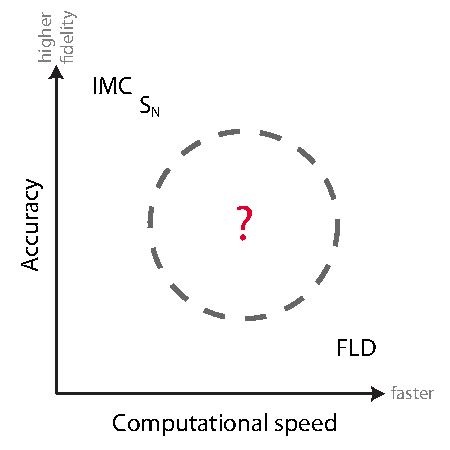
\includegraphics[width=3in]{fidelity}
  \caption{Figurative representation of existing TRT methods, showing the
  trade-off between accuracy and speed.}
  \label{fig:fidelity}
\end{figure}

With our development of anisotropic diffusion and its application to TRT, we
hope to provide a new solution process that is much less expensive than
full-fledged transport but more theoretically robust than standard diffusion or
FLD. Such a method would fit near the question mark in
Fig.~\ref{fig:fidelity}.

%%%%%%%%%%%%%%%%%%%%%%%%%%%%%%%%%%%%%%%%%%%%%%%%%%%%%%%%%%%%%%%%%%%%%%%%%%%%%%%%
\section{Synopsis}

The remainder of this thesis is organized into the following chapters.

\chaptersynopsis{chap:trtBackground}
The assertions about the difficulty of computational modeling of thermal
radiative transfer are explained by presenting the equations themselves. We give
a brief overview of existing approximations to the TRT equations and discuss how
those approximations are used in our work. Particular emphasis is given to the
semi-implicit treatment, which allows the nonlinear problem to be approximated
by a system of linear equations.

\chaptersynopsis{chap:adDerivation}
With the transport equation in hand, we derive a new approximation to radiation
transport, anisotropic diffusion. The derivation accounts for both time
dependence and boundary conditions. We then discuss some of the properties of
the AD method and make predictions for its range of applicability.

\chaptersynopsis{chap:aponeDerivation}
The derivation of the time-dependent AD equations assumed that the solution
changes slowly in time, which can be a poor approximation when applied to
TRT: it can actually lead to the nonphysical transfer of energy faster than the
speed of
light. This chapter addresses that shortcoming by modifying the ansatz used in
deriving the anisotropic diffusion equations, leading to a new ``anisotropic
\Pone'' method.

\chaptersynopsis{chap:implementation}
The leakage terms for anisotropic diffusion are more complex than standard
diffusion: rather than a scalar diffusion coefficient, AD has a diffusion
tensor. This necessitates unusual discretization schemes in all but the simplest
of problems. We present new discretization schemes for Cartesian \xy\ geometry
that can account for the transverse leakage induced by the anisotropic diffusion
tensor.

\chaptersynopsis{chap:flatland}
As mentioned earlier, the ``flatland'' geometry has recently proven to be a
valuable test bed for new transport methods because of its smaller phase space
and correspondingly easier solution. This chapter gives a thorough overview of
the differences between flatland and true 3-D geometries, with a focus on
implementing flatland solvers. We also explore diffusion in flatland, not only
deriving the prior result that the diffusion coefficient is different but also
formulating correct diffusion boundary conditions. Finally, we present the AD
equations in flatland geometry.

\chaptersynopsis{chap:simpleNumericalResults}
Before applying the anisotropic approximations to full nonlinear transport in
multi-dimensional geometries, it is important that we test individual components
of the derivation. We detail several steady-state problems that test the
discretization schemes, flatland diffusion boundary conditions, and anisotropic
diffusion boundary conditions. We also test some simple linear transport
problems.

\chaptersynopsis{chap:trtNumericalResults}
Finally, we test the applicability of the anisotropic methods to the nonlinear
TRT equations. To begin, we examine a few simple test problems in 1-D, where the
anisotropic methods merely ``smear'' the diffusion coefficients spatially.
This provides a test bed for determining the robustness of the nonlinear
treatment. Then
we move to more complicated flatland problems that simulate radiation flow
through an optically thin channel. (This is the qualitative configuration of
the CRASH problem.)
Additionally, we apply the AD method to some difficult 2-D problems in the
literature that feature optically thick obstacles rather than optically thin
streaming channels.

\chaptersynopsis{chap:conclusion}
The final chapter summarizes the results of the theory developed in this thesis
and its application to TRT problems. We discuss possible improvements to the new
methods and other future work.

